\documentclass{article}

% to compile a camera-ready version, add the [final] option, e.g.:
% \usepackage[final]{neurips_2019}

% to avoid loading the natbib package, add option nonatbib:
% \usepackage[nonatbib]{neurips_2019}

\usepackage[utf8]{inputenc} % allow utf-8 input
\usepackage[T1]{fontenc}    % use 8-bit T1 fonts / remove for ReScience
\usepackage{hyperref}       % hyperlinks
\usepackage{url}            % simple URL typesetting
\usepackage{booktabs}       % professional-quality tables
\usepackage{amsfonts}       % blackboard math symbols
\usepackage{nicefrac}       % compact symbols for 1/2, etc.
\usepackage{microtype}      % microtypography
\usepackage{amsmath}        % used for math symbols/equations
\usepackage{dsfont}         % imports Greek letter symbols
\usepackage{enumerate}      % other enumerate options
\usepackage{float}          % specific image placement
\usepackage{graphicx}       % enables images
\usepackage{caption}        % allows centered caption
\usepackage{subcaption}     % caption for subfigures
\usepackage[english]{babel}


% \usepackage[dvipsnames]{xcolor}   % remove for ReScience
\usepackage[normalem]{ulem}
\newif{\ifhidecomments}
\setcitestyle{authoryear,open={(},close={)}}

\title{[Re] Can gradient clipping mitigate label noise?}

% The \author macro works with any number of authors. There are two commands
% used to separate the names and addresses of multiple authors: \And and \AND.
%
% Using \And between authors leaves it to LaTeX to determine where to break the
% lines. Using \AND forces a line break at that point. So, if LaTeX puts 3 of 4
% authors names on the first line, and the last on the second line, try using
% \AND instead of \And before the third author name.

\author{
  David Mizrahi \\
  EPFL\\
  \texttt{david.mizrahi@epfl.ch} \\
  \And
  Oğuz Kaan Yüksel \\
  EPFL\\
  \texttt{oguz.yuksel@epfl.ch} \\
  \And
  Aiday Marlen Kyzy \\
  EPFL \\
  \texttt{aiday.marlenkyzy@epfl.ch} \\
}

\begin{document}

\maketitle



\section{Introduction}

Reproducibility is a key ingredient for an impactful scientific discovery, which allows future practitioners to build on the shoulders of published work. Reproducibility is also an important step to promote open and accessible research, allowing the scientific community to quickly integrate new findings and convert ideas to practice more seamlessly. In the spirit of promoting a culture of reproducible science in the Machine Learning community, we have hosted the fourth iteration of the ML Reproducibility Challenge in 2020. Unlike previous years, in this challenge we increased the scope to include a broad range of top Machine Learning conferences, including NeurIPS, ICML, ICLR, CVPR, ECCV, ACL and EMNLP. The goal of this challenge was to investigate the reproducibility of accepted papers published in these top conferences, and in-turn contribute to the better understanding of their central claims. In this special issue of ReScience C Journal, we present the peer-reviewed accepted papers of the 2020 ML Reproducibility Challenge.

\section{Challenge}

The goal of the challenge was to reproduce the central claims of papers published in top Machine Learning conferences of the year. Unlike the last iteration (NeurIPS 2019), in this year we focus on the central claim of the papers, and participants were open to choose to work on either all claims or partial claims depending on the complexity of the project. Participants were also free to reuse authors’ code when available, while being encouraged to explore beyond simply running the code provided to verify reproducibility. The challenge involved a “Claim paper” step, where early on  participants  were encouraged to submit a claim on the paper they wished to work on using the OpenReview portal. The objective of the claiming process was to help participants  narrow down their task by writing a short summary of items they wished to explore in reproducing the papers.

As in the last iteration, participants were free to claim multiple papers, and multiple teams could claim the same paper. In this year’s iteration, a total of 244 claims were submitted, which is a 41\% increase over last year. However, the total number of final submissions was slightly lower at 82 papers (vs 84 in previous year). We had participation from 48 institutions (47 universities and 1 industry organization). Top participating institutes consisted of University of Amsterdam, Netherlands, Indian Institute of Technology Gandhinagar, India, University of Waterloo, Canada, San Jose State University, USA. In these cases (and several others), a high participation rate occurred when a professor at the university used this challenge as a final course project.

It is also worth noting that this iteration of the challenge witnessed a significant jump in the quality of the reproducibility reports. After extensive peer review, in this special issue we present the top 23 accepted reports, selected from 82 submissions, thus driving up the acceptance rate from 11\% last year to 28\% this year.


\section{Reproducibility Summary and Template}

The substantial increase in the quality of the submitted reports is attributed to two key decisions: reducing the scope of the challenge to cover central claims of the paper, and introducing the Reproducibility Summary Template to help authors to communicate their results and findings clearly and concisely, given that scientific communication is challenging. While there are many different types of papers, there are also common elements across ML, NLP, and vision. In a reproduction report, the main emphasis is on good reporting.

This year we introduced a first-page summary and optional template. This template:
\begin{itemize}
  \item Has a place for reporting all items on the reproducibility checklist
  \item Acts as guide for researchers
  \item Shows that they understood the main claims, and the evidence that supports those claims.
  \item Allows readers to quickly look up what they're interested in -- readers know what sections to check
\end{itemize}

\section{Going beyond}

Another crucial factor contributing to the increase in quality of the reports is that this year’s edition saw many authors going above and beyond the original paper, running additional experiments and analyses and converting code between frameworks (e.g. Tensorflow → PyTorch). This was particularly encouraging since it is an indicator of the evolution of the Reproducibility Challenge from a simple replication of the initial results to a broader scope in terms of depth of engagement with reproducing research. We are impressed with the work of this year’s authors and look forward to seeing further developments of the challenge!


\section{Platforms}

This challenge is conducted with the support of PapersWithCode and OpenReview. PapersWithCode is an open, collaborative platform to discover latest trending machine learning research papers with their codebases, which enables rapid re-usability and reproducibility of published works. PapersWithCode enabled us to reach a wide audience of students and researchers who participated in the competition. As last time, OpenReview provided crucial logistic support by providing an unique platform to claim and submit reproducibility reports. After submission, all reports went through a thorough peer review process consisting of hundreds of reviewers from the Machine Learning community, and OpenReview provided an easy-to-use platform for managing reviews and administrative processes. Finally, we used a public Github repository to perform the final editorial process of converting accepted papers into ReScience format, and thereby publish 23 high quality reports in this special issue.


\section{Conclusion}

Reproducibility of central claims of papers published in Machine Learning conferences has been a center of considerable attention over the past several years. Conferences such as NeurIPS, ICLR, AAAI, ICML, EMNLP have routinely included reproducibility workshops and challenges to cultivate the culture of reproducible science in the community. Several conferences have also introduced code submission policies and Reproducibility Checklists to further advance the cause and build momentum of reproducible science. We hope our continued endeavour of hosting regular reproducibility challenges and publishing high-quality peer-reviewed reproducibility reports will contribute more information about the existing published papers, and help strengthen their core contributions in the process, while also promoting open, accessible and sound machine learning research.

\section{Acknowledgements}

We thank the board and program committee of NeurIPS, ICML, ICLR, ACL, EMNLP, CVPR and ECCV for partnering with us in this massive initiative and supporting the challenge. We thank the OpenReview team (in particular Andrew McCallum, Parag Pachpute, Melisa Bok, Celeste Martinez Gomez, Pam Mandler and Mohit Uniyal) for their constant support in hosting and building the customized portal used in our challenge. We thank Robert Stojnic, Ross Taylor and Elvis Saravia from PapersWithCode for hosting and supporting the challenge along with its logistics. We thank the ReScience board (in particular Nicolas Rougier, Konrad Hinsen and Olivia Guest) for presenting the accepted reports in their esteemed journal. Finally, we thank all of our participants who dedicated time and effort to verify results that were not their own, to help strengthen our understanding of the concepts presented in the papers.  A special thank you to Ana Lucic (University of Amsterdam), who instructed and supported several of the student teams whose reports are featured in this issue.

\section{Reviewers}

Our reviewers need a special section dedicated to thank them for their tireless efforts in screening and providing valuable feedback to the Area Chairs to select the best papers. We were fortunate enough to attract a large pool of reviewers, who spent their precious time to critically review the reports. We would like to specifically acknowledge  our Emergency reviewers (marked in *) who responded to our call for help to review some additional reports at the last minute. We hope that our reviewer base will keep supporting us in this endeavour in future.

\begingroup
\fontsize{8pt}{8pt}\selectfont
\begin{multicols}{3}
\begin{itemize}[label={}]
\item Abhinav Agarwalla
\item Akshita Gupta
\item Ali Hürriyetoğlu
\item Andreas Ruttor
\item Andrew Drozdov
\item Anis Zahedifard
\item Arna Ghosh
\item Azin Shamshirgaran
\item Bharathi Srinivasan *
\item Chao Qin
\item Charbel Sakr
\item Chuan Li
\item Clement Laroche
\item David Arbour
\item Di He
\item Dmitriy Serdyuk
\item Donghyeon Cho
\item Dylan Hadfield-Menell
\item Emmanuel Bengio
\item Ernest K. Ryu
\item Fan Feng
\item Fatemeh Koochaki
\item Fernando Martínez-Plumed
\item Gagana B
\item Georgios Leontidis
\item Haitian Sun
\item Hanna Suominen
\item Hao He
\item Heng Fang
\item Huaibo Huang
\item Huseyin Coskun
\item Ishani Vyas
\item Jiakai Zhang
\item Jiangwen Sun
\item Jie Fu
\item Jitong Chen
\item John Frederick Wieting
\item Kanika Madan
\item Katherine Lee
\item Kaushy Kularatnam
\item Koustuv Sinha *
\item Leo M Lahti
\item Leonid Kholkine
\item Levent Sagun
\item Li cheng
\item Lijun Wu
\item Linh Tran *
\item Lluis Castrejon
\item Mahzad Khoshlessan
\item Maneesh Kumar Singh
\item Mani A,Marija Stanojevic
\item Maria Maistro
\item Marija Stanojevic
\item Marin Misur
\item Massimiliano Mancini
\item Matthew Kyle Schlegel
\item Matthew Ryan Krause
\item Maxime Wabartha
\item Maxwell D Collins
\item Md Imbesat Hassan Rizvi
\item Melanie F. Pradier
\item Michal Drozdzal
\item Mingrui Liu
\item Monjoy Saha
\item Neal Fultz
\item Nikolaos Vasiloglou
\item Olga Isupova *
\item Olivier Delalleau
\item Opeyemi Osakuade
\item Otasowie Owolafe *
\item Pablo Robles-Granda
\item Pascal Lamblin
\item Patrick Philipp
\item Paul Tylkin
\item Peter Henderson
\item Prasad Sudhakara Murthy
\item Praveen Narayanan
\item Radha Chitta
\item Rajanie Prabha
\item Sadid A. Hasan
\item Samira Shaikh
\item Sandhya Prabhakaran
\item Satya Prakash Dash
\item Seohyun Kim
\item Sepehr Janghorbani
\item Shuai Kyle Zheng
\item Siwei Wang
\item Steffen Udluft
\item Sunnie S. Y. Kim
\item Swetha Sirnam *
\item Tammo Rukat
\item Taniya Seth
\item Tobias Uelwer
\item Ujjwal Verma
\item Vibha Belavadi
\item Víctor Campos
\item Wenbin Zhang
\item Wenhao Yu
\item Xavier Bouthillier
\item Xavier Sumba
\item Xiang Zhang
\item Xiao Zhang
\item Xin Guo
\item Yufei Han
\item Yuntian Deng
\item Zhangjie Cao
\end{itemize}
\end{multicols}
\endgroup

% Emergency Reviewers: Linh Tran,Olga Isupova,Swetha Sirnam,Bharathi Srinivasan,Otasowie Owolafe, Koustuv Sinha



% All Reviewers: Marin Misur, Abhinav Agarwalla, Akshita Gupta, Ali Hürriyetoğlu, Andreas Ruttor, Andrew Drozdov, Anis Zahedifard, Arna Ghosh, Azin Shamshirgaran, Chao Qin, Charbel Sakr, David Arbour, Di He, Dmitriy Serdyuk, Donghyeon Cho, Dylan Hadfield-Menell, Emmanuel Bengio, Ernest K. Ryu, Fan Feng, Fernando Martínez-Plumed, Gagana B, Georgios Leontidis, Haitian Sun, Hanna Suominen, Hao He, Heng Fang, Huaibo Huang, Huseyin Coskun, Ishani Vyas, Jiakai Zhang, Jiangwen Sun, Jie Fu, Jitong Chen, John Frederick Wieting, Kanika Madan, Katherine Lee, Kaushy Kularatnam, Leo M Lahti, Leonid Kholkine, Levent Sagun, Li cheng, Lijun Wu, Lluis Castrejon, Mahzad Khoshlessan, Maneesh Kumar Singh, Maria Maistro, Marin Misur, Massimiliano Mancini, Matthew Kyle Schlegel, Matthew Ryan Krause, Maxime Wabartha, Maxwell D Collins, Md Imbesat Hassan Rizvi, Michal Drozdzal, Mingrui Liu, Monjoy Saha, Nikolaos Vasiloglou, Olivier Delalleau, Pablo Robles-Granda, Pascal Lamblin, Patrick Philipp, Paul Tylkin, Peter Henderson, Praveen Narayanan, Radha Chitta, Rajanie Prabha, Sadid A. Hasan, Samira Shaikh, Sandhya Prabhakaran, Sepehr Janghorbani, Shuai Kyle Zheng, Siwei Wang, Steffen Udluft, Sunnie S. Y. Kim, Tammo Rukat, Taniya Seth, Tobias Uelwer, Ujjwal Verma, Vibha Belavadi, Víctor Campos, Wenbin Zhang, Wenhao Yu, Xavier Bouthillier, Xavier Sumba, Xiang Zhang, Xin Guo, Yufei Han, Yuntian Deng, Zhangjie Cao, Chuan Li, Melanie F. Pradier, Marija Stanojevic, Clement Laroche, Fatemeh Koochaki, Mani A,Marija Stanojevic, Neal Fultz, Opeyemi Osakuade, Prasad Sudhakara Murthy, Satya Prakash Dash, Seohyun Kim, Xiao Zhang.


\bibliographystyle{plainnat}
\bibliography{bibliography}

\appendix
\section{Alternative iFlow model}
A comment in the files mentioned an error in the implementation because the Softplus function was applied to $\xi$ as well as $\eta$ from the natural parameters $\mathbf{\lambda (u)}$. An alternative version of the implementation was also tested where the Softplus activation function was only exerted on $\xi$, as there are no constraints on the sign of $\eta$. 

% MCC of 0.72 (0.057)
The results obtained using this method were approximately the same as the original performance of the iFlow. A mean MCC of 0.72 with a standard deviation of 0.057 was achieved. Because these results were not a significant improvement, it was decided to include this experiment as an appendix.  

\section{Baseline improvement experiments}

The table below shows the results of experiments with changing the iVAE architecture to increase complexity. As shown, adding skip connections or layer normalisation to the architecture did not increase performance with respect to the unchanged baseline. Due to the high training time, no additional experiments could be done.

\label{sec:baselineexperiments}
\begin{center}
\begin{tabular}{ccccc} 
     \toprule
     addition & NUM\_HIDDEN & NUM\_LAYERS & AVG MCC \\
     \midrule
     - & 50 & 3 & 0.483 (\textpm 0.059)\\
     residual connections & 50 & 3 & 0.474 (\textpm 0.053)\\
     layer normalisation & 50 & 3 & 0.461 (\textpm 0.051)\\
     \bottomrule\\
\end{tabular}
\end{center}

\newpage
\section{Visualizations for Fixed iVAE}
\label{sec:appendixC}

\begin{figure}[ht]
    \centering
    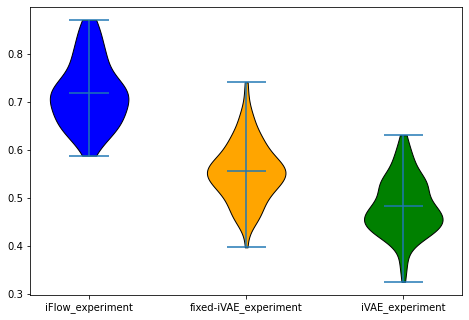
\includegraphics[width=0.5\textwidth]{Reproducibility_Challenge_2020/IMG/scores/violin_plot_fixed.png} 
    \caption{Alternative visualisation of the MCC scores obtained by the models, including the fixed iVAE.} 
    \label{fig:violinplot} 
\end{figure}

\begin{figure}[ht]
    \centering
    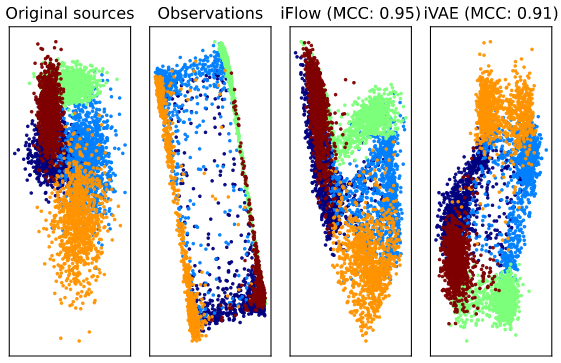
\includegraphics[width=0.5\textwidth]{Reproducibility_Challenge_2020/IMG/2D_perf/2D_performance_fixed_iVAE.png} 
    \caption{Visualisation of 2D-cases, comparing iFlow to the fixed version of iVAE.} 
    \label{fig:fixedMCCscores} 
\end{figure}

\begin{figure}[!htbp]
    \centering
    \begin{minipage}[b]{\textwidth}
        \centering
       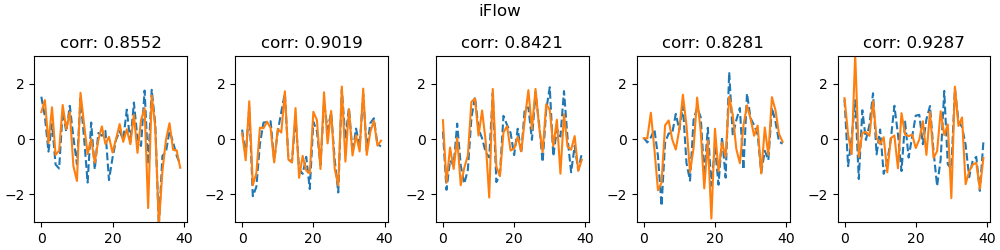
\includegraphics[width=0.8\textwidth]{Reproducibility_Challenge_2020/IMG/latent_corr/best_iFlow_42.png}
    \end{minipage}
    \begin{minipage}[b]{\textwidth}
    \centering
       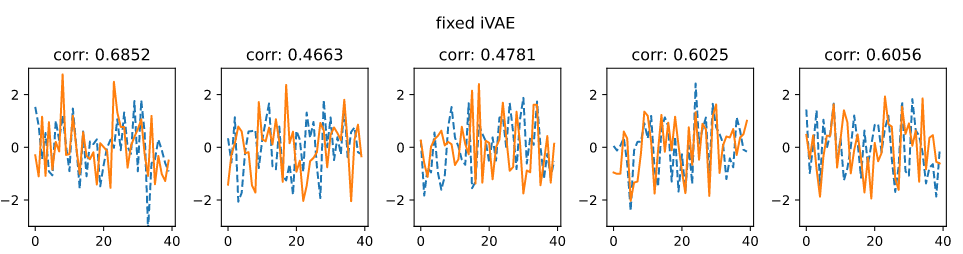
\includegraphics[width=0.8\textwidth]{Reproducibility_Challenge_2020/IMG/latent_corr/fixed_iVAE_42.png}
    \end{minipage}
    \caption{Comparison of the latent variables recovered by the models (orange lines) to the true latent variables (dashed blue lines) for individual dimensions. This figure shows results for the seed that resulted in the best iFlow performance.}
    \label{fig:latentcorr_fixed1}
\end{figure}

\begin{figure}[!htbp]
    \centering
    \begin{minipage}[b]{\textwidth}
        \centering
       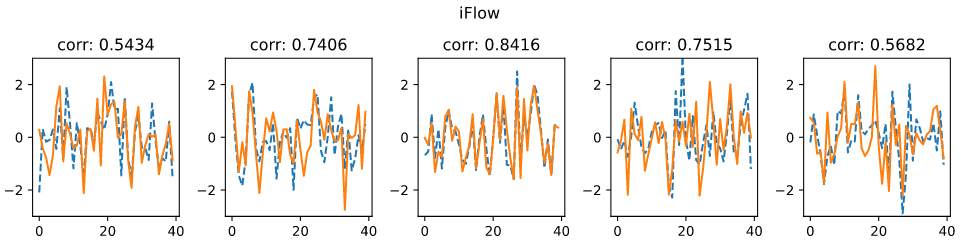
\includegraphics[width=0.8\textwidth]{Reproducibility_Challenge_2020/IMG/latent_corr/iFlow_X.png}
    \end{minipage}
    \begin{minipage}[b]{\textwidth}
    \centering
       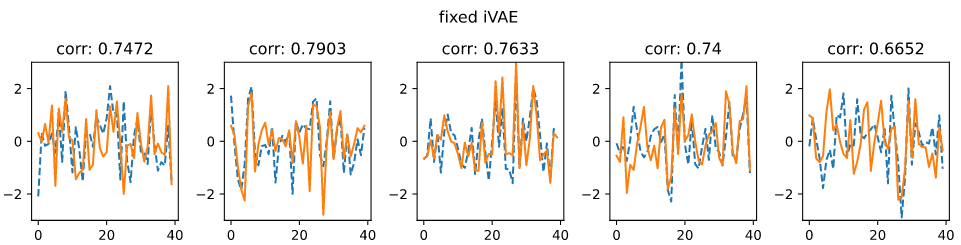
\includegraphics[width=0.8\textwidth]{Reproducibility_Challenge_2020/IMG/latent_corr/best_fixed_iVAE_X.png}
    \end{minipage}
    \caption{Comparison of the latent variables recovered by the models (orange lines) to the true latent variables (dashed blue lines) for individual dimensions. This figure shows results for the seed that resulted in the best fixed iVAE performance.}
    \label{fig:latentcorr_fixed2}
\end{figure}


\end{document}